\section{Contextual analyser}
\label{background:checker}

\subsection{Symbol table}
\label{sec:bg:symbol-table}
Most programming languages allow declarations and a usage of symbolic names (identifiers) to represent constants, variables, functions, types and objects. The compiler checks that these names are used correctly and according to the programming language definition. \cite[p. 179]{craftingCompiler}

\par
We assume that the abstract syntax tree (AST) has been constructed. We then perform a pass over the AST to process symbol declarations and connect each symbol reference with its declaration. Symbol references are connected with declarations through a symbol table. An AST node that mentions a symbol by name is enriched with a reference to the name’s entry in the symbol table. If such a connection cannot be made, then the reference is improperly declared and an error message is issued. Otherwise, subsequent passes can use the symbol table reference to obtain information about the symbol. \cite[p. 180]{craftingCompiler} 

\par 
Different pieces of information may be associated with an identifier - it can have various attributes. Attributes of an identifier usually include anything the compiler knows about it and the main source of these attributes are declarations. Identifiers are used in many different ways in various languages, including variables, constants, types, procedures, classes, and fields. Every identifier, therefore, will not have the same set of attributes associated with it. \cite[p. 298]{craftingCompiler} 

\subsection{Scope rules}
Scopes are offered by various programming languages to constrain the usage of a symbol name to a given region in a program. \cite[p. 282]{craftingCompiler} 

\par
Static scoping is employed by most modern programming language due to its clarity - a programmer can anticipate the behaviour of a variable in the scope without understanding context. In a statically scoped languages, references are resolved to the declaration in their closest containing scope. For example, if a language utilizes static scoping, a call of a function $\textit{g}$ in the following pseudo code would evaluate to 10.

\begin{lstlisting}[]
    int x = 10
    function f(){
        x
    }
    function g(){
        int x = 20;
        f()
    }
\end{lstlisting}

\par 
On the other hand, in a dynamic scope environment, the resolution of references depends on the execution context. This means that when looking for variable $x$ in the above example, calling functions are searched. Therefore, a call of a function $\textit{g}$ would evaluate to 20. 

\par 
For such block structured languages, there are two common approaches for implementing a symbol table. Either a symbol table may be associated with each scope or all symbols may be entered in a single, global table. A single symbol table must accommodate multiple, active declarations of the same symbol. \cite[p. 285]{craftingCompiler} 

\subsection{Type checking}

\par 
Among the attributes mentioned in
\cref{sec:bg:symbol-table}, are types. To verify that types in the program are properly issued, we perform another pass over the AST. The primary activities of this pass will be constructing a symbol table structure that represents all of the declarations in the tree and performing type checks as necessary. \cite[p. 300]{craftingCompiler} 
\par 
The different checks mirror the semantic rules defined in \cref{sec:design:formal:type-system}. The type check of a literal node is trivial since the type is immediately available. To type check an identifier, we simply look up its type in a symbol table and issue an error in case it cannot be found. A more complex expression, for example, one constructed with usage of a binary operator, can be typed checked by obtaining the types of both the left expression and the right expression. The type checking depends on the operator and types of operands. The following is an AST representation of binary expression: \cite[p. 329]{craftingCompiler} 

\begin{figure}[!ht]
  \centering
  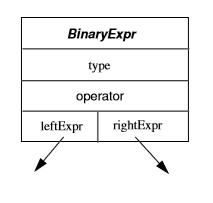
\includegraphics[scale=0.8]{Pictures/AST-B-Exp.png}
  \caption{AST representation of a binary expression}
  \label{fig:ast-binary-expression}
\end{figure}


\newblock
\par
A concrete example is checking the expression $\textit{e}$: $5 + 6$ - we first check the types of operands and learn that both are $\textit{integers}$. Since the operator is a plus, we can type check expression $e$ as $integer$. Type checking is further described in section \cref{sec:design:formal:type-system}.

